\section{測定環境}
    サンプルの測定に使用した希釈冷凍機はBLUE Fors LD250である。希釈冷凍機の冷却原理を簡潔に説明する\cite*{fridge,fridge2}。希釈冷凍機は1K Spot、Still(分流器)、Mix Chamber(混合器)の大別して3つの部屋で構成されている。
    \begin{figure}[H]
        \begin{minipage}[t]{0.6\columnwidth}
            \centering
            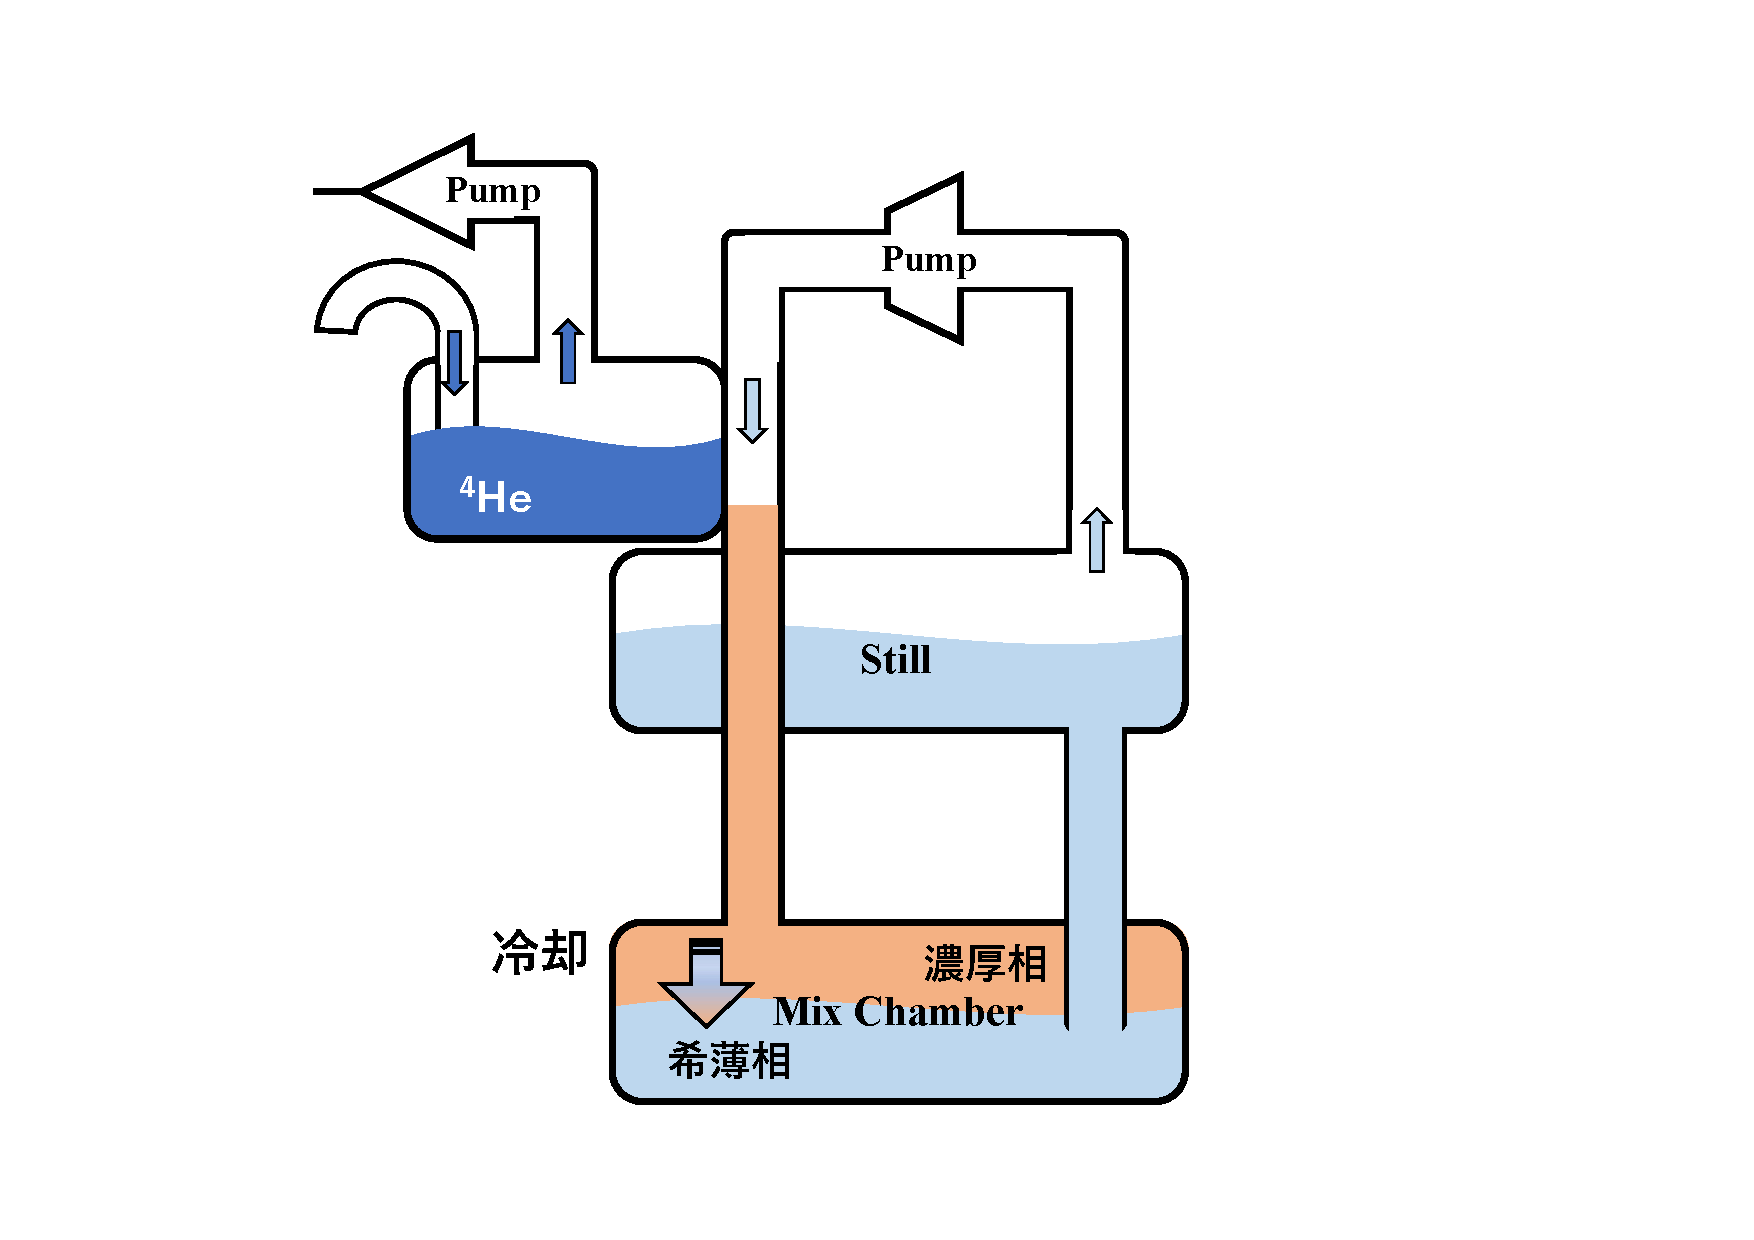
\includegraphics[clip, width=1.0\columnwidth]{fridge.pdf}
            \caption{希釈冷凍機の基本原理}
        \end{minipage}%
        \begin{minipage}[t]{0.4\columnwidth}
            \centering
            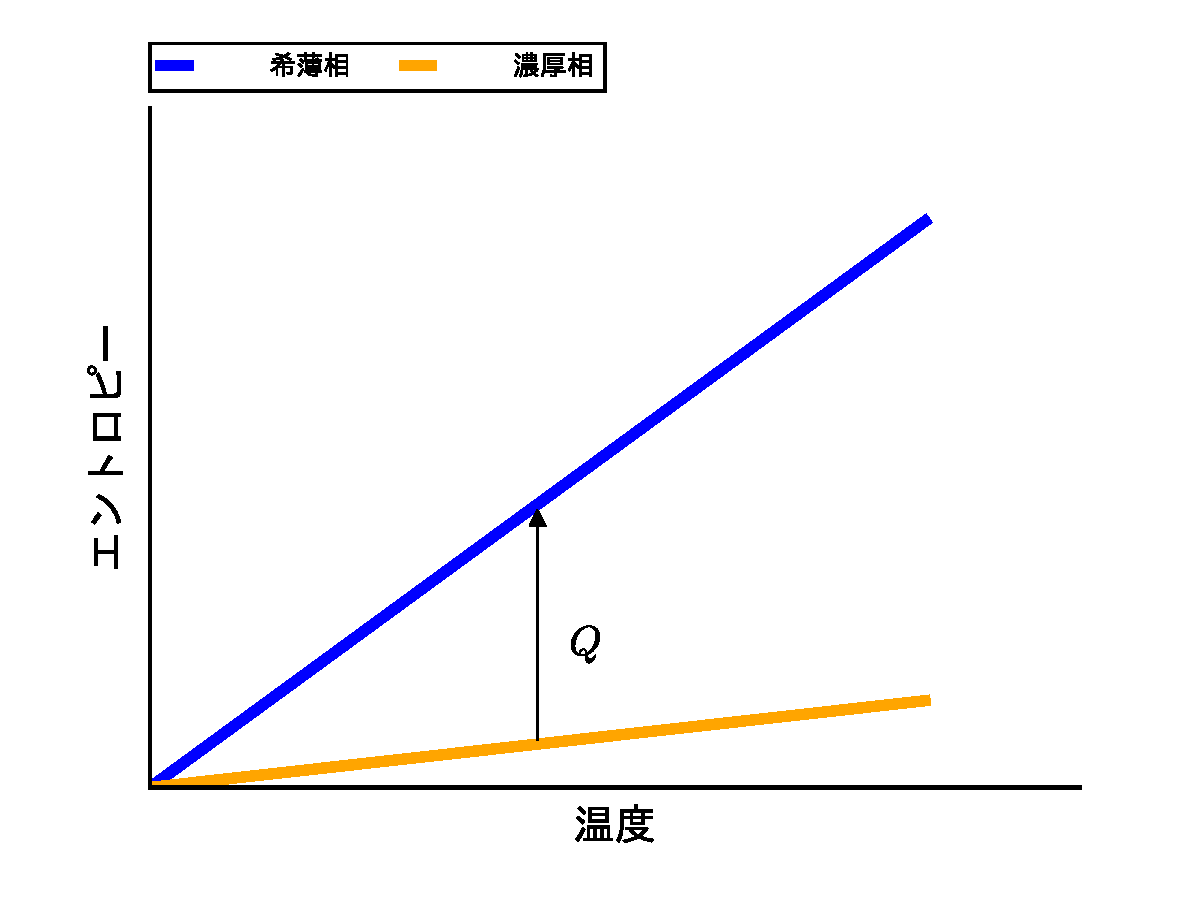
\includegraphics[clip, width=1.0\columnwidth]{entropy.pdf}
            \caption{濃厚相と希薄相のエントロピー}
        \end{minipage}
    \end{figure}
    1K Spot内にはHe4が充填されており排気冷却を行うことで最低温度1Kを実現している。1K Spotの主な役割はHe3を液状にするため冷却機である。次にMix Chamberであるが、この容器内ではHe3とHe4が相分離した状態で混合されている。He3の濃度の小さい相を希薄相、大きな相を濃厚相と呼ぶ。このMix Chamber が希釈冷凍機能を持った心臓部である。希釈冷凍機を構成する最後の1つ、StillではHe3の排気が行われている。冷却の基本原理はHe3を選択的に排気することでHe3を濃厚相から希薄相へと強制的に’蒸発’させることにより生まれる断熱減圧冷却法であるが、STillには希薄相のみが充填されており、He3が選択的に排気されている。右の図では濃厚相と希薄相では希薄相の方がエントロピーの違いを示している。希薄相の方が濃厚相よりもエントロピーが高いため、He3が濃厚相から希薄相へと浸透するとよってHe3外部空から熱を吸収するため,冷却が起こる。排気したHe3は再び濃厚相へと供給され、この繰り返しにより冷凍機内部は10mKまで冷却される。希釈冷凍機の図にあるように、冷凍機内部にはいくつものプレートで区切られており、プレートの熱伝導を利用して、各ステージは段階的に温度が代わっている。最下部のCold Finger内にサンプルを搭載する。サンプルはパーマロイでできた$\mu$metalで蔽うことで外部磁場を遮蔽している。
    \begin{figure}[H]
        \centering
        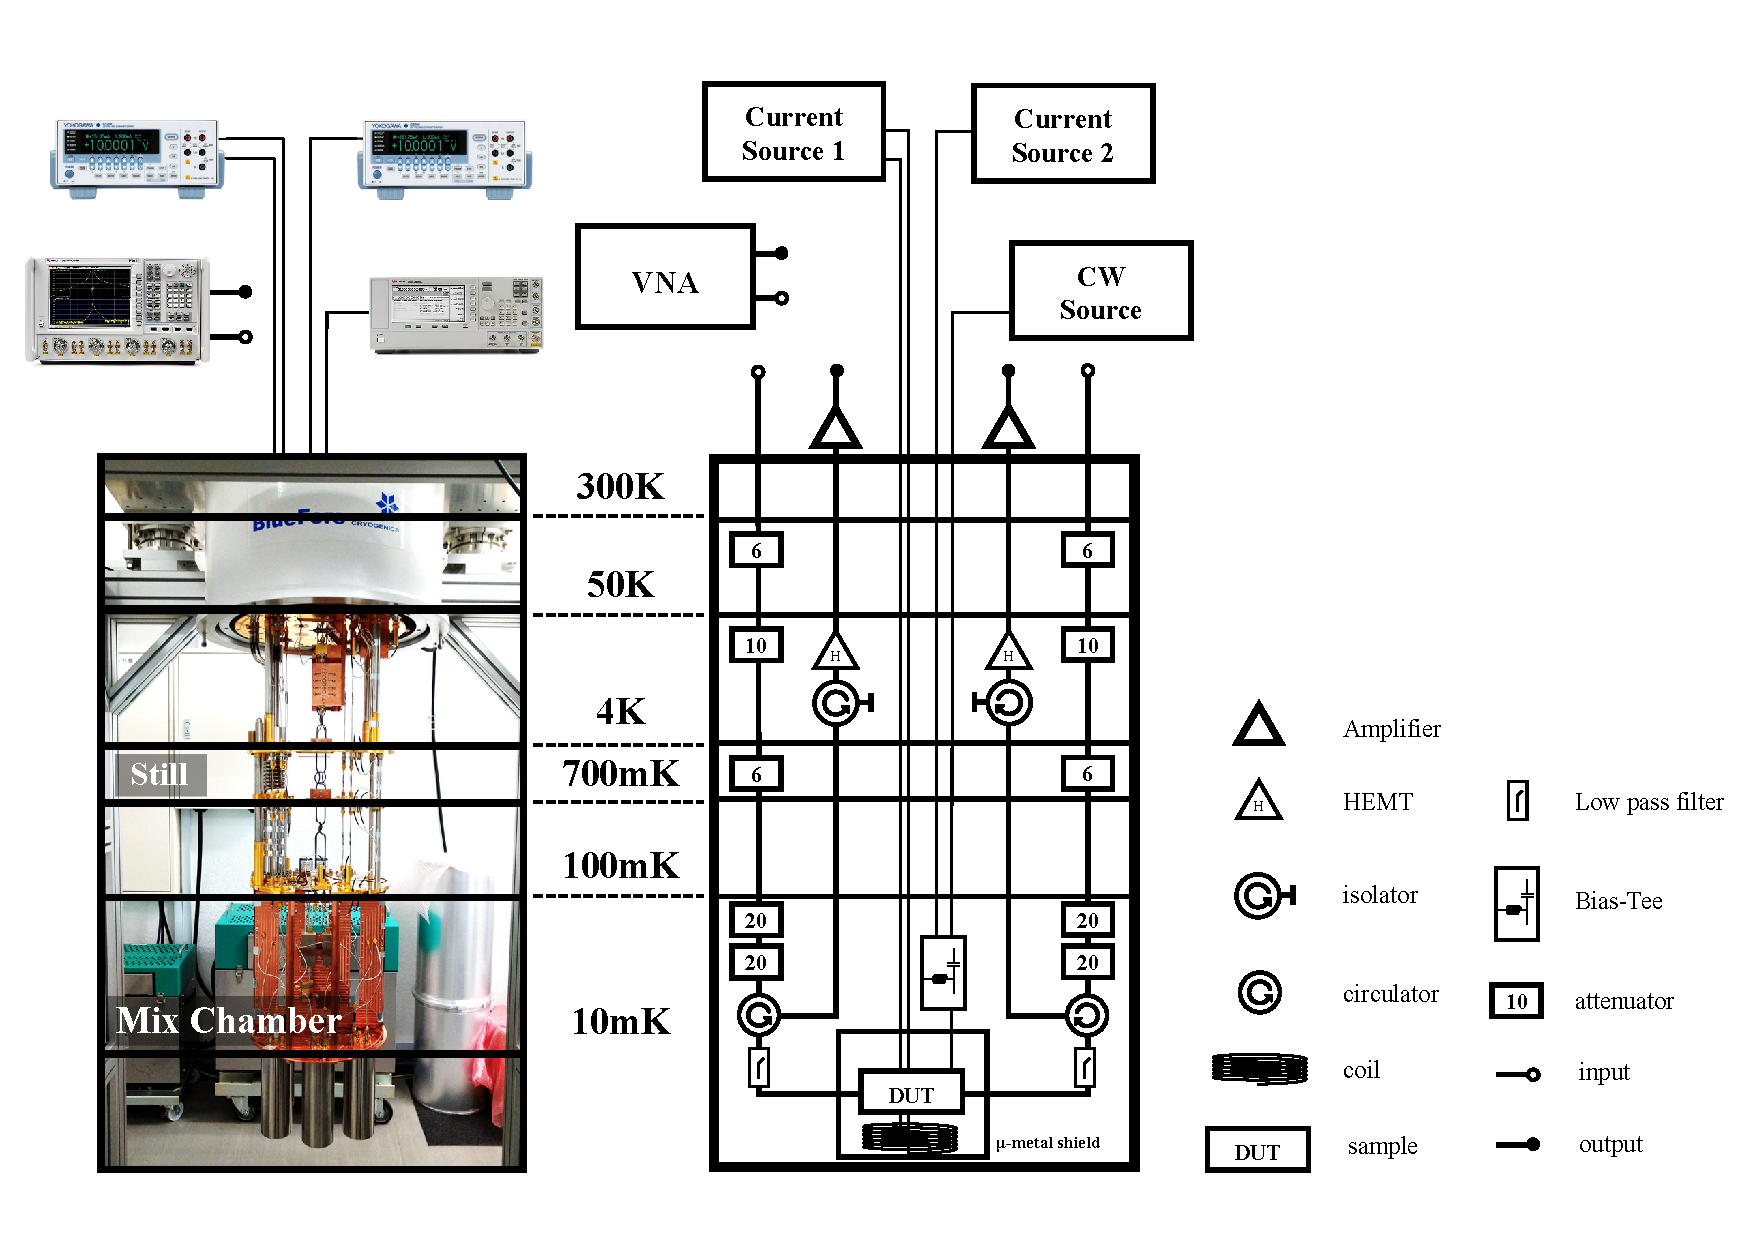
\includegraphics[width=11cm,angle=-90]{fridgesetup2.pdf}
        \caption{希釈冷凍機のセットアップ}
    \end{figure}
    冷凍機内部の部品はアンプやサンプルホルダーに至るまでインピーダンスが50$\Omega$となるように適切に設計、製造されたものを使用している。
    本実験で使用した機材はKeysight社のN5231A PNA-Lマイクロ波ネットワーク・アナライザ、13.5 GHz及びE8257D PSGアナログ信号発生器、100 kHz~67 GHz、横河電気の直流電圧/電流源 GS200である。電流源はサンプルホルダーに搭載されたコイル操作用、サンプルに搭載されたオンチップバイアスラインを操作用の2つを使用した。サンプル自体には2つのポートが存在するが、4~8GHz帯のCirculatorを取り付けることで透過測定及び反射測定が可能となっている。すなわちVNAとサンプルの接続方法は4通り存在し、それぞれについて測定を行った。
    \begin{figure}[H]
        \begin{minipage}[t]{0.5\columnwidth}
            \centering
            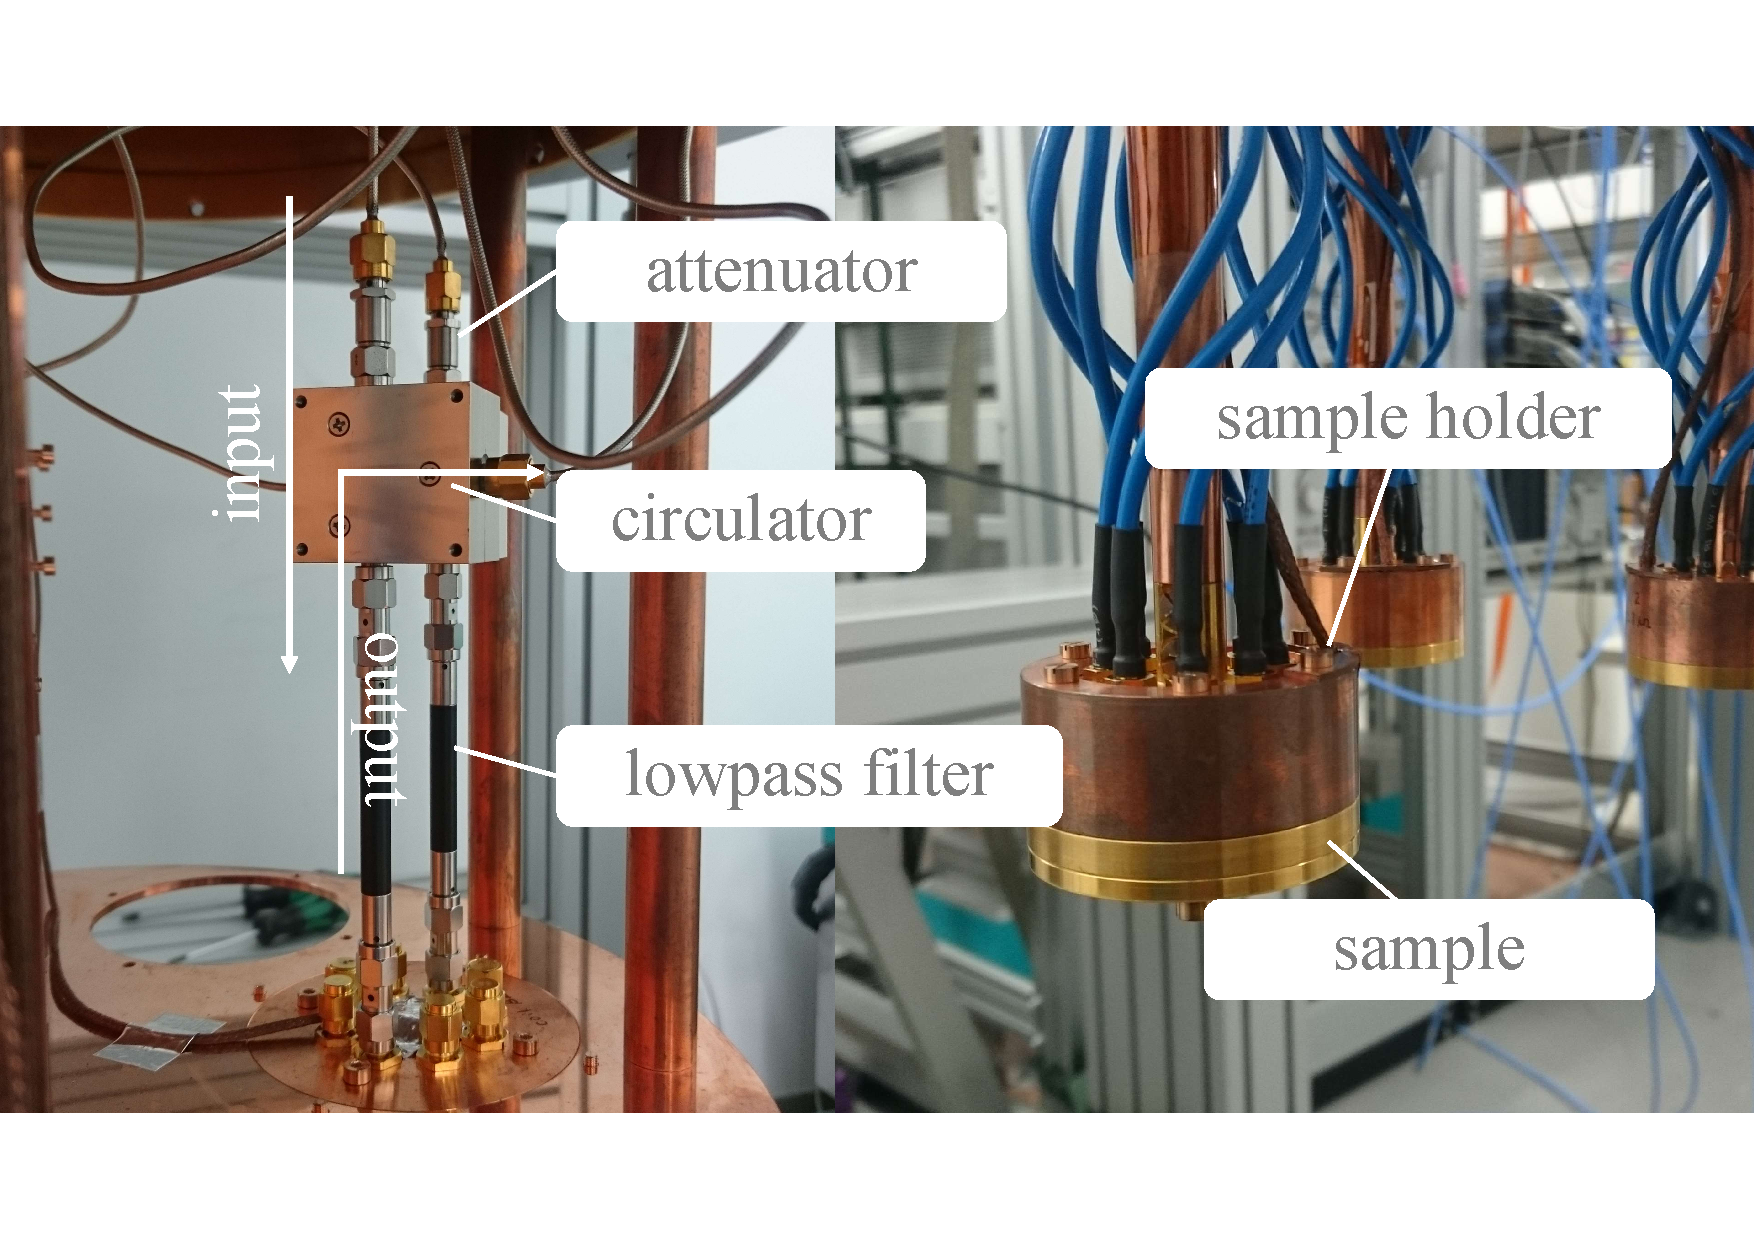
\includegraphics[clip, width=1.0\columnwidth]{samplesetup.pdf}
            \caption{希釈冷凍機内のサンプルセットアップ}
        \end{minipage}%
        \begin{minipage}[t]{0.5\columnwidth}
            \centering
            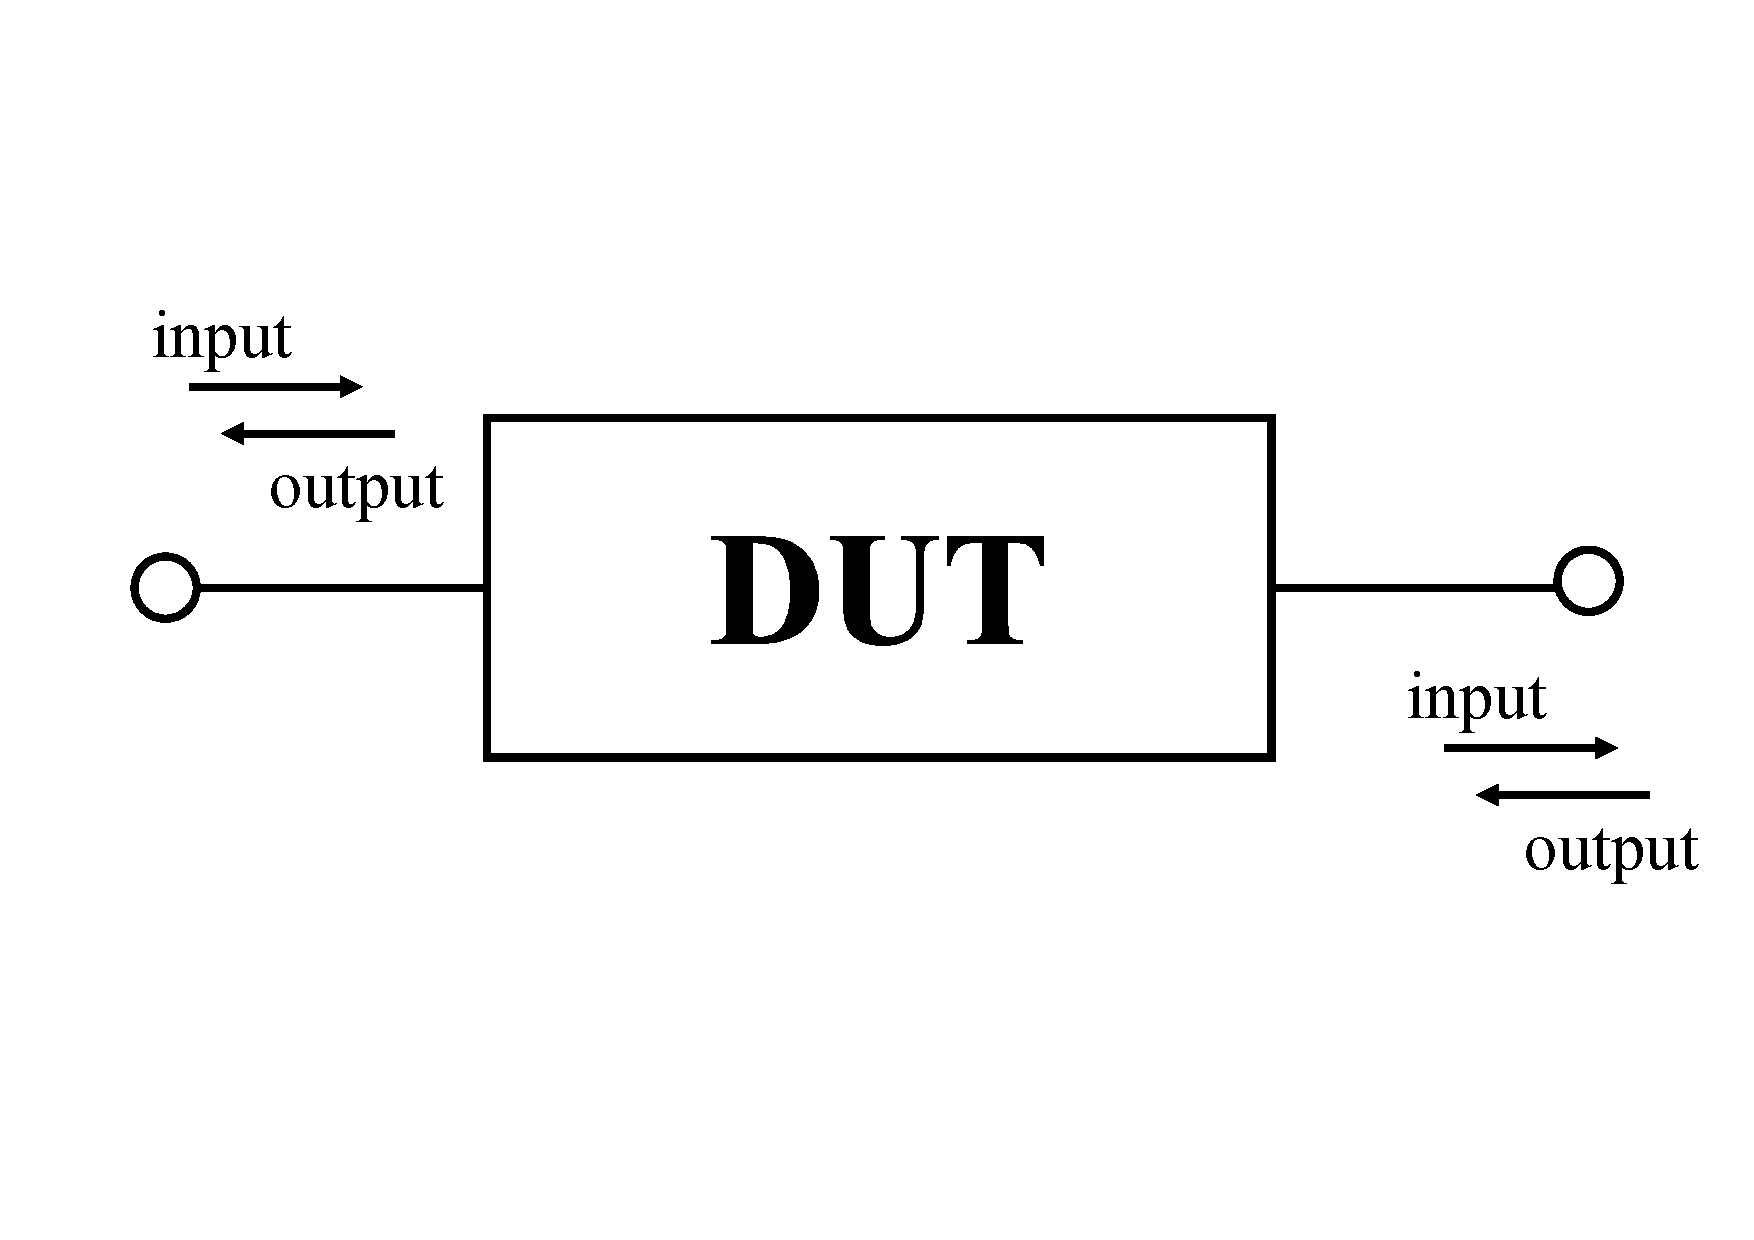
\includegraphics[clip, width=1.0\columnwidth]{inputoutput.pdf}
            \caption{測定方法}
        \end{minipage}
    \end{figure}
    また、冷凍機内には62dBのAttenuator(減衰器)が取り付けられており、ケーブルの減衰7dBも含めるとVNAから出力される信号は総計69dB減衰されることに注意する。

    次にサンプルについて説明する。サンプルとPCBはAlの細線を用いてボンディングされている。サンプルのグランド及びPCBからサンプルへの伝送ラインの接続はこのAl細線により確保されている。
    \section{LEAl,LEJの測定結果}
    \section{LEMの測定結果}
        \subsection{スクリーニングパラメータβの変調}
        LEMの結合性能を評価する前に、dc-SQUIDのチューニングを行う必要がある。前章に記載したように、サンプルホルダーに搭載された外部コイルを操作することで、サンプル全体に均一磁場を印加することができる。均一磁場はメインループ、サブループを貫く磁束の数は面積比に比例する。設計では、メインループ:サブループ=1:100としているため、サブループを貫く磁束のスケールで測定を行えば、dc-SQDUIの影響をよくみることができる。
        電流源であるGS200のオンチップバイアスをオフに、コイルにに依るグローバルバイアスをスイープしながらVNAによるonetonespectroscopyを行うと次のような測定結果を得る。
        \begin{figure}[H]
            \begin{minipage}[t]{0.5\columnwidth}
                \centering
                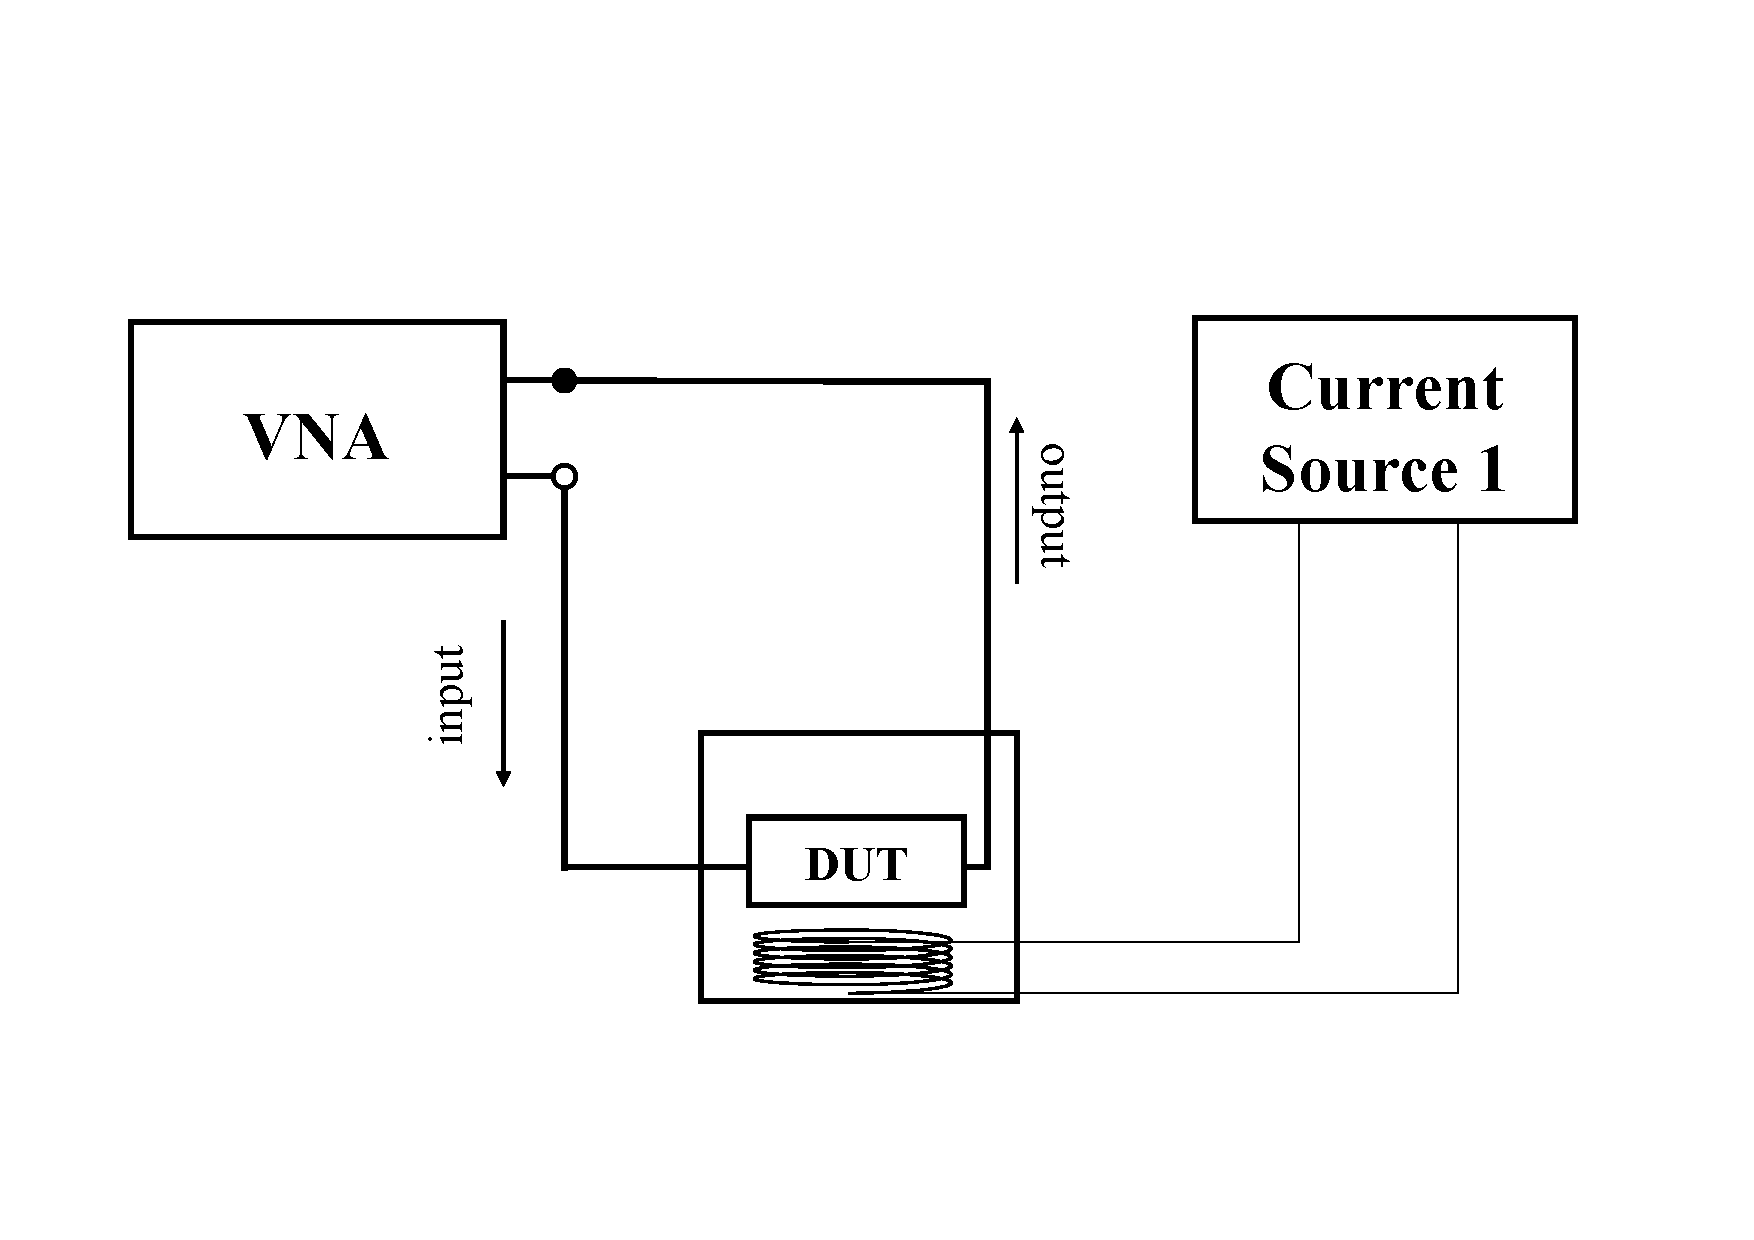
\includegraphics[clip, width=1.0\columnwidth]{globalscan.pdf}
                \caption{希釈冷凍機内のサンプルセットアップ}
            \end{minipage}%
            \begin{minipage}[t]{0.5\columnwidth}
                \centering
                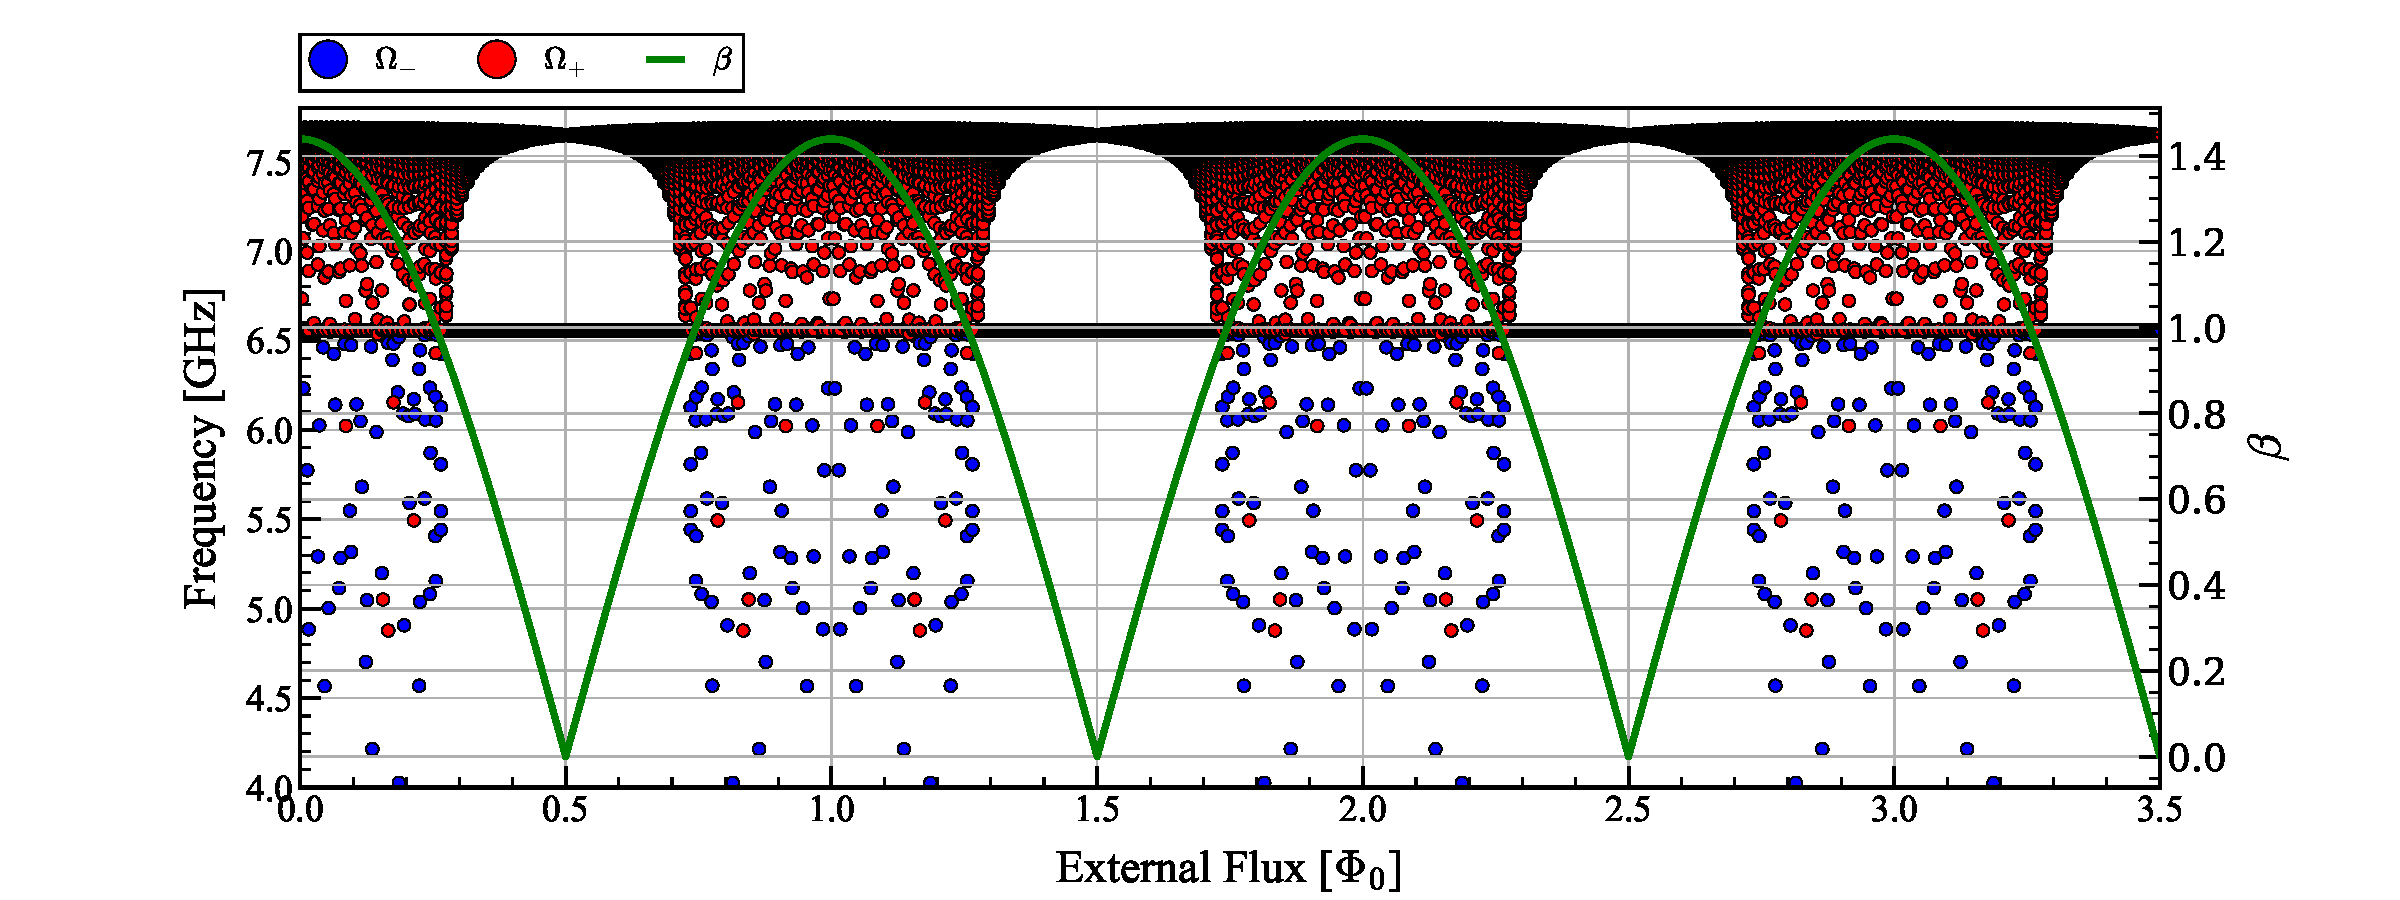
\includegraphics[clip, width=1.0\columnwidth]{compoundeigen6.pdf}
                \caption{測定方法}
            \end{minipage}
        \end{figure}
        
        \begin{figure}[H]
            \centering
            \includegraphics[width=14cm]{compoundeexp.pdf}
            \caption{測定結果}
        \end{figure}
        一見すると離散的な振る舞いをしているが、これは横軸の点数が不足しているためであり、区間[0,1]におけるプロットをみると連続的であることがわかる。
        \begin{figure}[H]
            \centering
            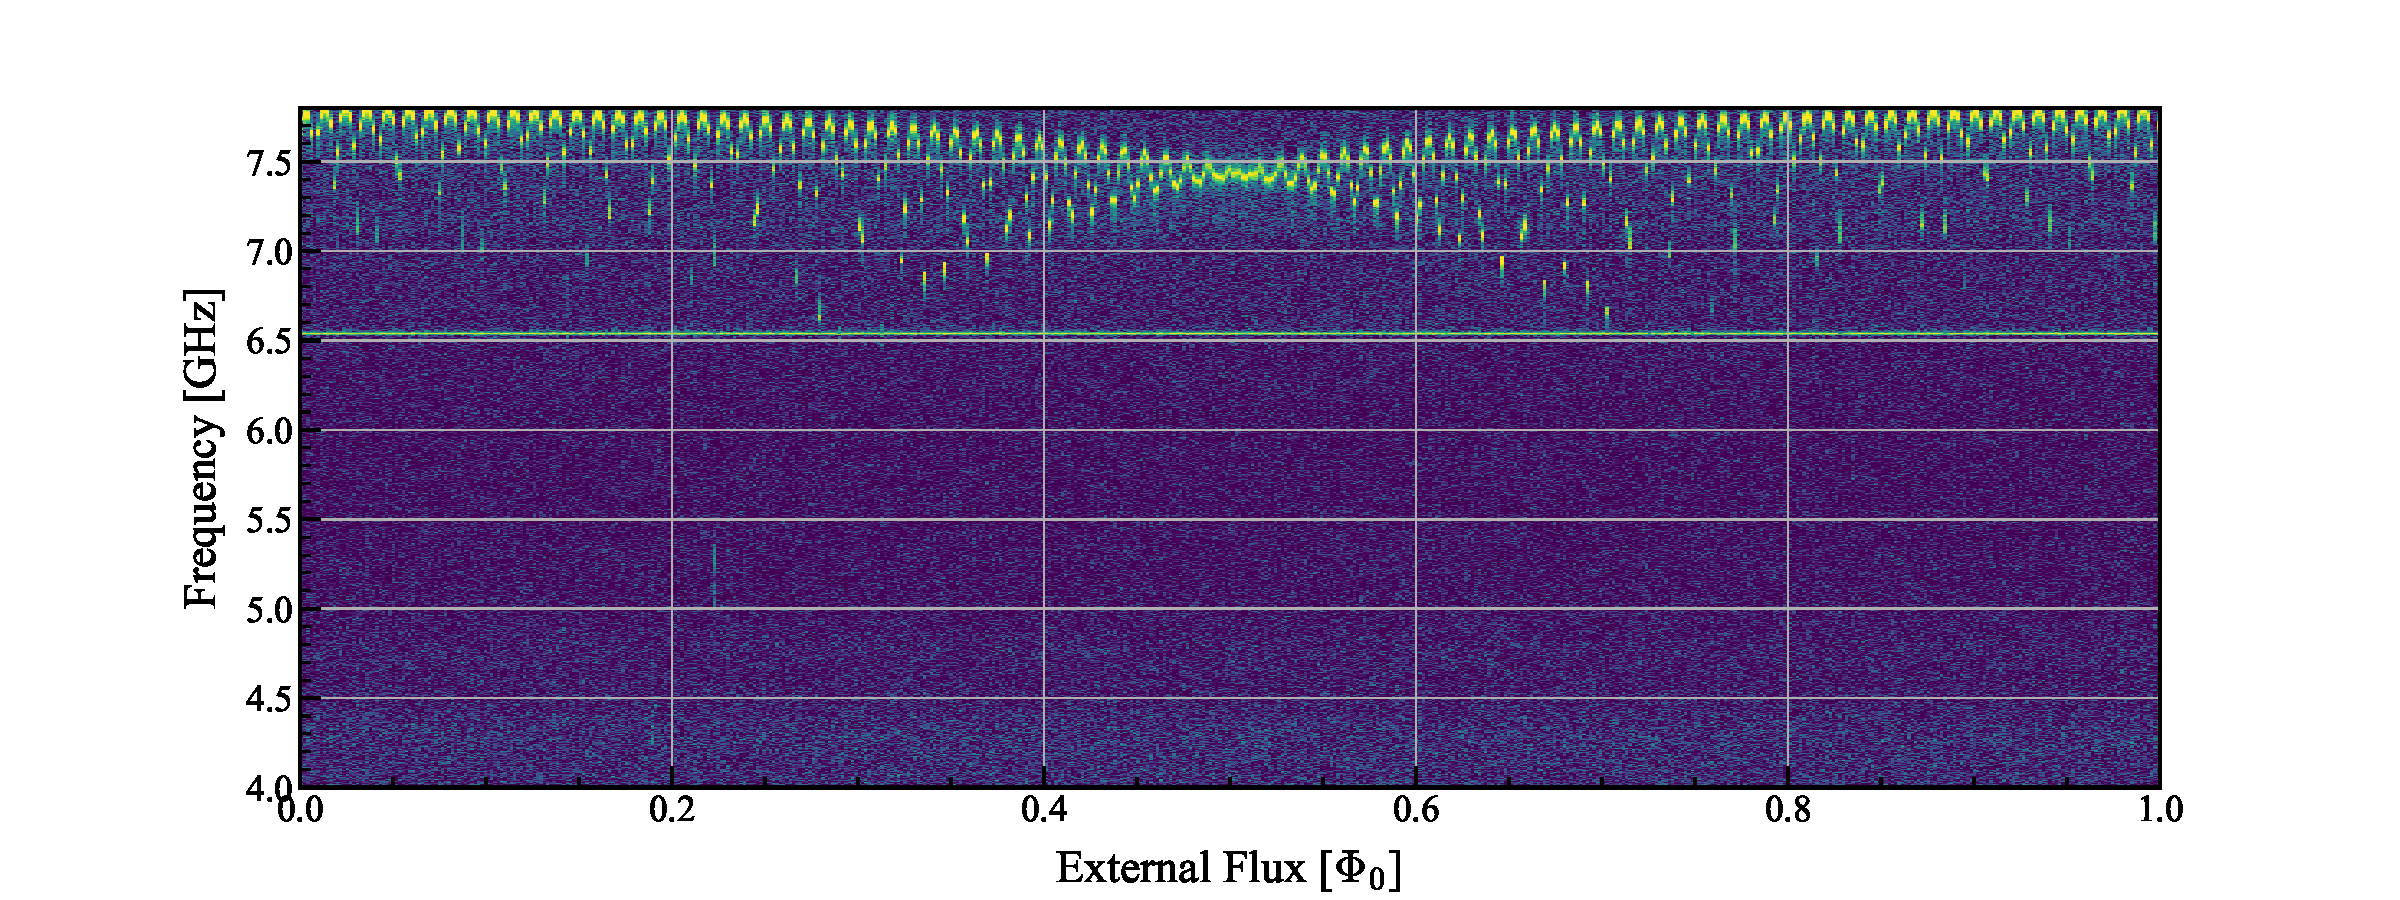
\includegraphics[width=14cm]{compoundeexp_zoom.pdf}
            \caption{測定結果}
        \end{figure}
        のようになる。
        続いてローカルバイアスによるサブループへのクロストークを計算する。ある区間におけるグローバルバイアスを各ローカルバイアス毎に計算すればよい。これによりローカルバイアスからグローバルバイアスへの相互インダクタンスMlsは00であると求まる。
        \subsection{スクリーニングパラメータβの変調}
        次にあるグローバルバイアスで固定した状態でローカルバイアスのみをスイープする。ローカルバイアスからグローバルバイアスへのクロストークが小さければスクリーニングパラメータβの値は一定となるため、十分広いローカルバイアスの区間でもスペクトルは一定となることが予想される。
        \begin{figure}[H]
            \centering
            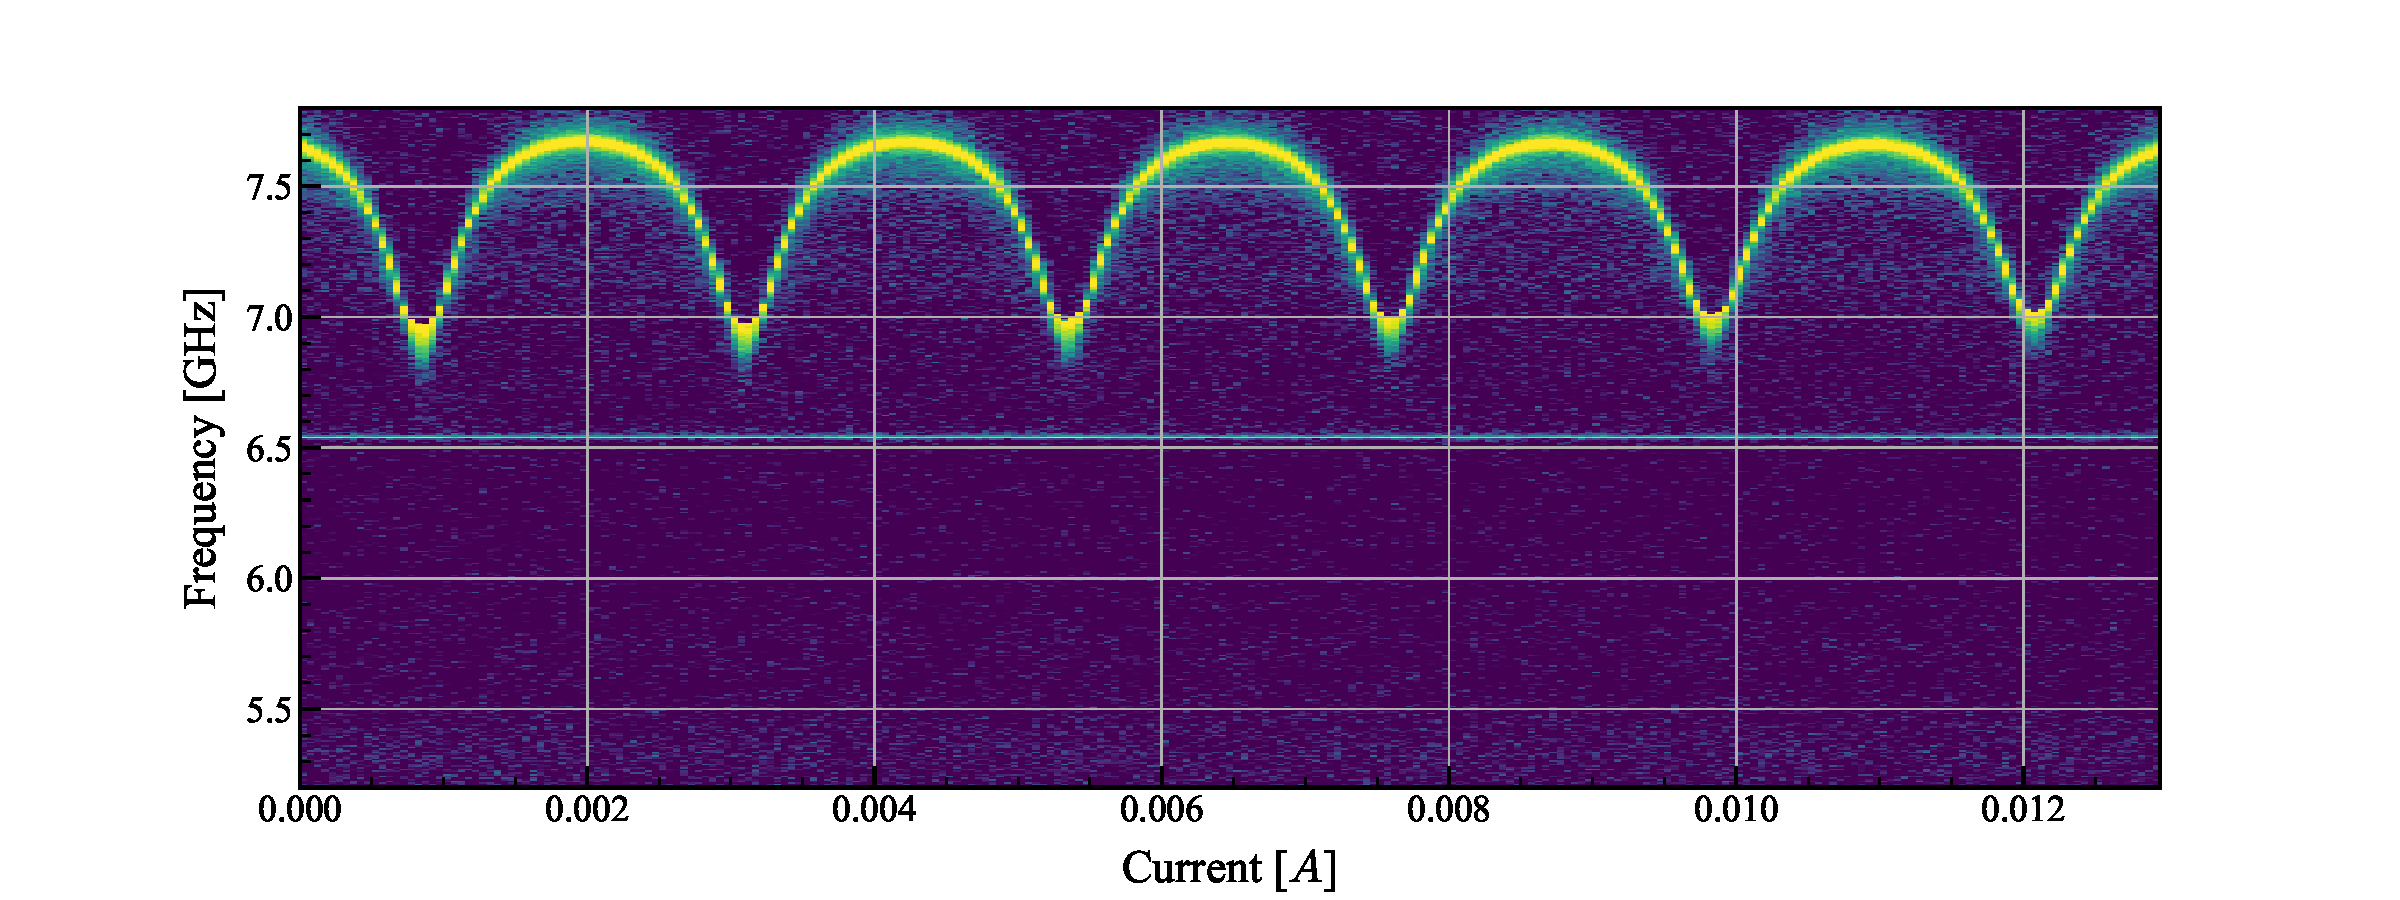
\includegraphics[width=14cm]{11.pdf}
            \caption{測定結果}
        \end{figure}
        クロストークによる若干の影響はみられるものの、1磁束区間に於けるスクリーニングパラメータβの変化量は微小であるといえる。各磁束バイアスからのクロストークを見積もれば電流限を同時に操作することで下図に示すようにスクリーニングパラメータβの値を一定に保ちつつメインループの磁束量を変えることができる。

    % \begin{figure}[H]
    %     \centering
    %     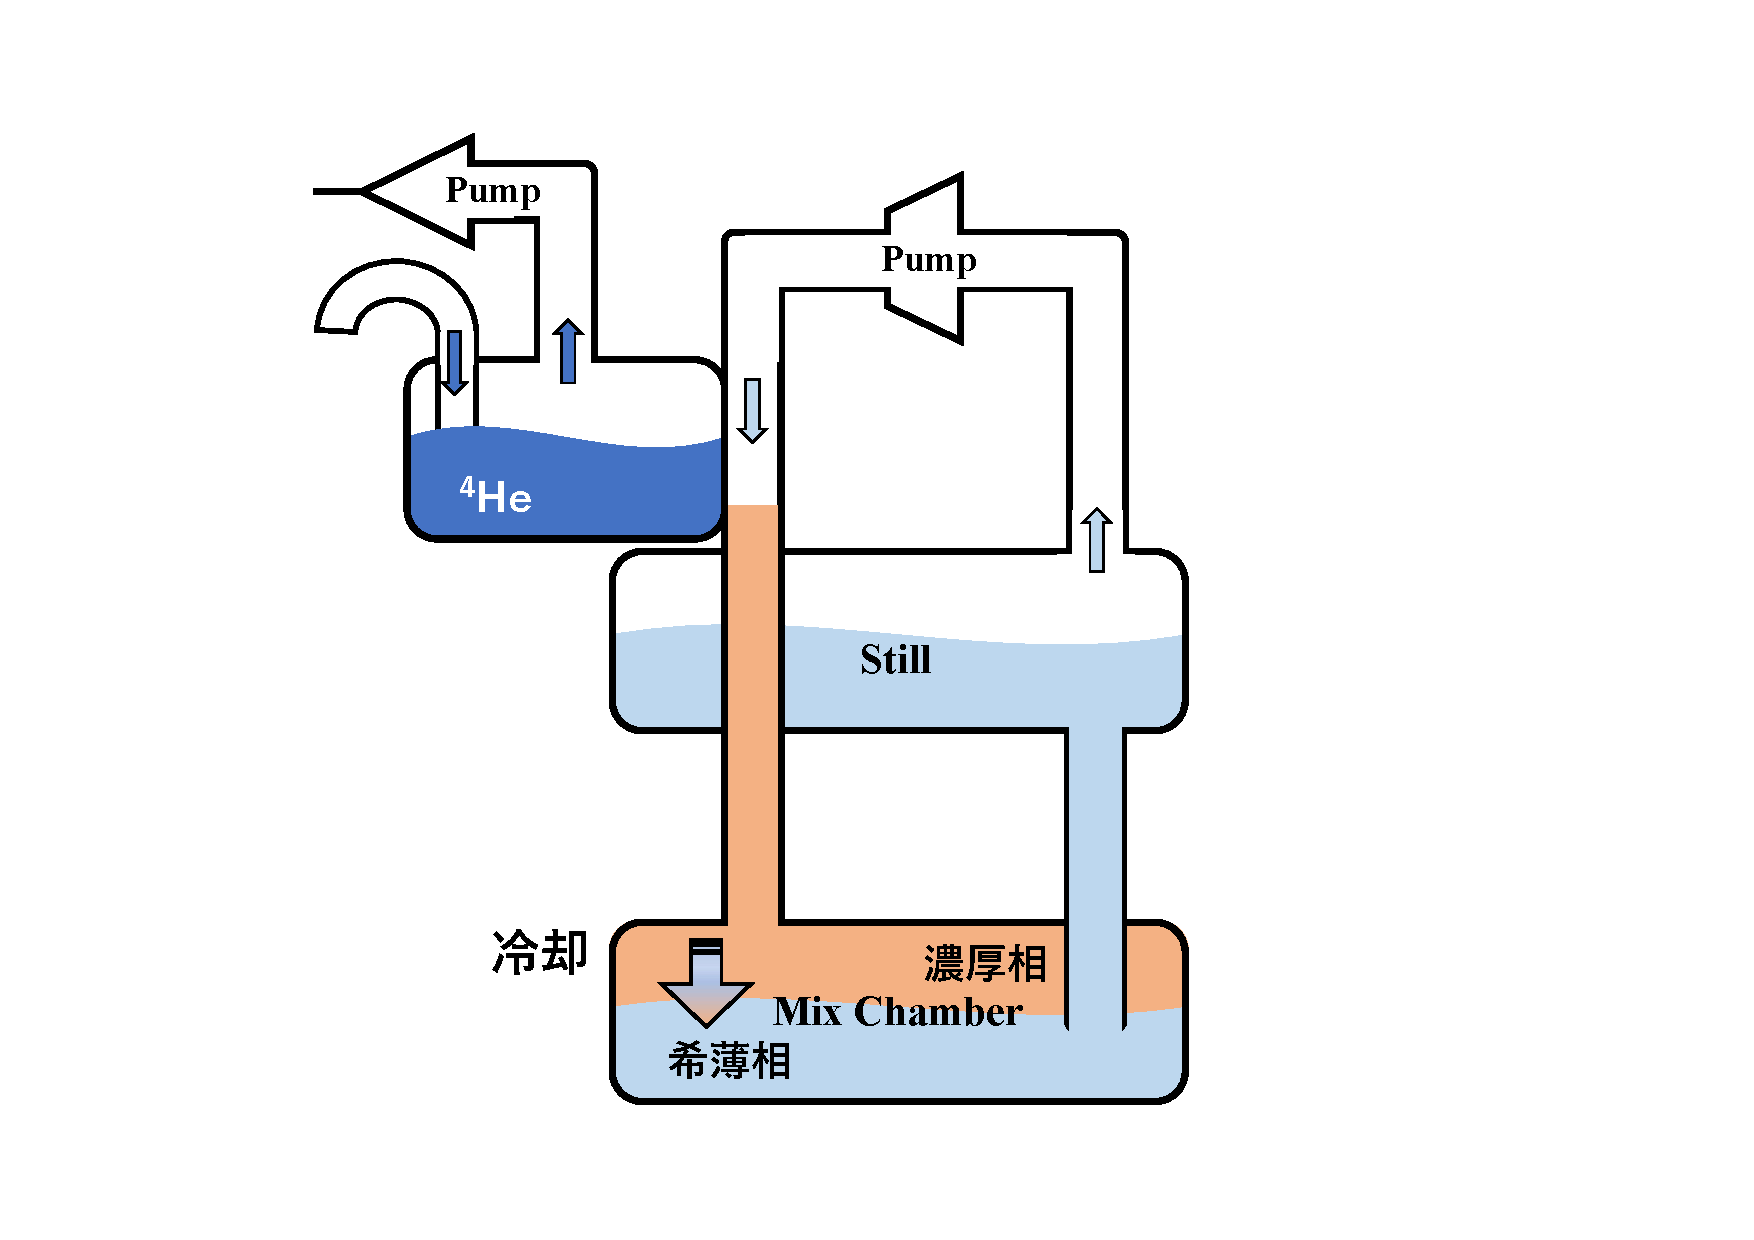
\includegraphics[width=4cm]{fridge.pdf}
    %     \caption{希釈冷凍機のセットアップs}
    % \end{figure}
